\section{Genetic Algorithms}
1975 yılında Michigan Üniversitesi'nden, psikolog ve bilgisayar bilimleri uzmanı J. H. Holland tarafından ortaya atılmıştır. Genetik algoritmalar, en iyinin korunması ve doğal seçilim ilkesinden esinlerek tasarlanmış bir optimizasyon ve arama yöntemidir. Rastlantısal olarak seçilen belli bir büyüklükte popülasyon oluşturulur. Popülasyondaki her birey kaynak için rekabet eder ve çiftleşir. Başarılı olanların (daha iyi uyum sağlayan) daha fazla yavru yapmak için çiftleşir. Başarılı olanlardan gelen genler nesilleri boyunca aktarılır. 

\begin{figure}[h]
    \centering
    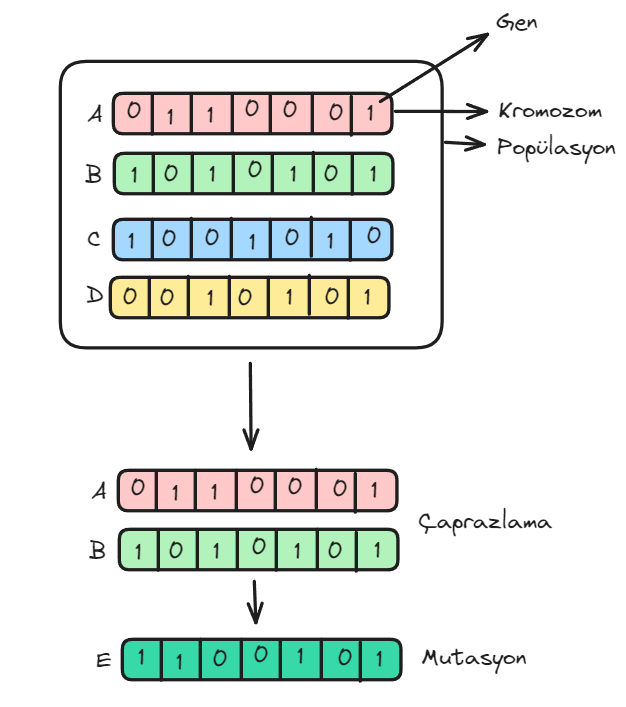
\includegraphics[width=1\textwidth]{images/genetic_algorithm.png}
    \caption{Genetik algoritma.}
    \label{fig:enter-label}
\end{figure}

\subsection{Çalışma Adımları}
\begin{enumerate}
    \item \textbf{Başlangıç Popülasyonunun Oluşturulması:} İlk olarak, rastgele veya belirli bir kriterlere göre oluşturulan bir popülasyon (bireylerin kümesi) seçilir.
    \item \textbf{Uygunluk Değerlerinin Hesaplanması:} Her birey için uygunluk değeri (fitness value) belirlenir. Bu değer, bireyin çözümünün ne kadar iyi olduğunu ölçer. Uygunluk değerleri, çözümün amacına bağlı olarak farklı şekillerde tanımlanabilir.
    \item \textbf{Seçim (Selection):} Yüksek uygunluk değerlerine sahip bireyler, gelecek nesle taşınacak olan ebeveynler olarak seçilir. Seçim süreci, bireylerin uygunluk değerlerine göre olasılıkla gerçekleştirilir.
    \item \textbf{Çaprazlama (Crossover):} Seçilen ebeveyn bireyler, genetik bilgi değişimi için çaprazlama işlemine tabi tutulur. Bu işlem, ebeveynlerin genetik materyallerini birleştirerek yeni bireyler (çocuklar) oluşturur.
    \item \textbf{Mutasyon (Mutation):} Yeni oluşturulan bireyler, belirli bir olasılıkla mutasyona uğratılır. Mutasyon, bireylerin genetik materyallerinde rasgele değişiklikler yaparak çeşitliliği arttırır.
    \item \textbf{Yeni Popülasyonun Oluşturulması:} Çaprazlama ve mutasyon sonucunda elde edilen yeni bireyler, eski popülasyonun yerini almak üzere bir sonraki nesil popülasyonunu oluşturur.
    \item \textbf{Durdurma Kriterlerinin Kontrol Edilmesi:} Belirli bir durma kriteri sağlanana kadar 2-6. adımlar arasındaki işlemler tekrarlanır. Durdurma kriteri, önceden belirlenmiş bir iterasyon sayısı, maksimum uygunluk değeri veya başka bir kriter olabilir.
\end{enumerate}

\subsection{Operatörler}
\begin{itemize}
    \item \textbf{Seçim (Selection):} Seçim operatörü, bir popülasyon içinden uygun bireyleri belirlemek için kullanılır. Bu operatör, bireylerin uygunluk değerlerine göre seçim yapar. Yüksek uygunluk değerlerine sahip bireylerin seçilme olasılığı daha yüksektir.
    \item \textbf{Çaprazlama (Crossover):} Çaprazlama operatörü, seçilen ebeveyn bireylerin genetik materyallerini birleştirerek yeni bireyler (çocuklar) oluşturur. Bu operatör, genetik çeşitliliği artırmak ve yeni çözümler üretmek için kullanılır.
    \item \textbf{Mutasyon (Mutation):} Mutasyon operatörü, çaprazlama sonucu oluşturulan yeni bireylerin genetik materyallerinde rasgele değişiklikler yapar. Bu değişiklikler, çeşitliliği artırır ve yeni çözümler üretmek için kullanılır.
\end{itemize}

\newpage